%\documentclass[handout,xcolor=pdftex,dvipsnames,table]{beamer}
\documentclass[10pt,xcolor=pdflatex,dvipsnames,table]{beamer}
\usepackage[cache=false]{minted}
\usepackage{tikz}
\usetikzlibrary{arrows,shapes}
\usepackage{fontawesome}
\usepackage{pgfpages}

\usetheme[numbering=none,progressbar=head,block=fill]{metropolis}
%\setbeamertemplate{footline}[text line]{A Sample Talk}
% Just insert the note text, no fancy hints.
%\setbeamertemplate{note page}[plain]
%\setbeameroption{show notes on second screen}

% Use modern fonts
\usefonttheme{professionalfonts}
\usepackage{unicode-math}
\setmainfont{FiraGO}[Scale = 1.0]
\setsansfont{FiraGO}
\setmonofont{Fira Mono}

\title{Building embedded systems using Elixir}
\subtitle{An introduction to Nerves and Phoenix Framework}
\date{Jul 17, 2019}
\author[Milton Mazzarri]{Milton Mazzarri \\
  \alert{milmazz @ \faTwitter \hspace{1pt} \faGithub \hspace{1pt} \faLinkedin}
}
\institute{Houston Functional Programmers Group}

\hypersetup{
	colorlinks=true,
	linkcolor=blue,
	pdfauthor={Milton Mazzarri},
	pdftitle={Building embedded systems with Elixir}
}

\newcommand\encircle[1]{%
	\tikz[baseline]
	\node[fill=orange, shape=circle, inner sep=0] (c#1) {\color{white}\strut #1};}

% To fix bug related to notes on second page
\makeatletter\def\beamer@framenotesbegin{% at beginning of slide
  \usebeamercolor[fg]{normal text}
  \gdef\beamer@noteitems{}%
  \gdef\beamer@notes{}%
}
\makeatother

% See: https://tex.stackexchange.com/questions/165929/semiverbatim-with-tikz-in-beamer
\makeatletter
\global\let\tikz@ensure@dollar@catcode=\relax
\makeatother

	\begin{document}
	% For every picture that defines or uses external nodes, you'll have to
	% apply the 'remember picture' style. To avoid some typing, we'll apply
	% the style to all pictures.
	\tikzstyle{every picture}+=[remember picture]

	\maketitle

	\section{Introduction}

	\begin{frame}
		\frametitle{Goals}

		\begin{itemize}
			%\item Introduction to Elixir, Nerves and Scenic Framework
      \item Introduction to Elixir and Nerves
			\item Boot a Raspberry Pi to an IEx prompt
			\item Boot a Raspberry Pi 3 B+ to an IEx prompt
			%\item Build a touch screen that runs Scenic Framework
		\end{itemize}
	\end{frame}

	\note{
	\small
		Hello everyone, my name is Milton Mazzarri and my goal today is to talk
		about how we can use Elixir to build and deploy bulletproof embedded systems,
		we will start talking about Nerves and also Scenic framework.
	}

  \section{Definitions}

  \begin{frame}
    \frametitle{Nerves}

    Nerves defines a new way to build embedded systems using Elixir. It's
    specifically designed for embedded systems, not desktop or server systems.
    Nerves is composed by three parts:

    \begin{description}[<alert@+>]
      \item[Platform] a customized, minimal Buildroot-derived Linux that boots
        directly to the BEAM VM
      \item[Framework] ready-to-go library of Elixir modules to get you up and
        running quickly
      \item[Tooling] powerful command-line tools to manage builds, update
        firmware, configure devices, and more
    \end{description}
  \end{frame}

  \begin{frame}
    \frametitle{Host}

    The computer on which you are editing source code, compiling, and
    assembling firmware
  \end{frame}

  \begin{frame}
    \frametitle{Target}

    The platform for which your firmware is built (for example, Raspberry Pi,
    Raspberry Pi 2, or Beaglebone Black)

    \begin{figure}
      \centering
      \includegraphics[width=.8\textwidth]{./figures/raspbp-overview}
      \caption{Raspberry Pi 3 Model B+\label{fig:raspbp-overview}}
    \end{figure}
    {\footnotesize Source: \href{https://www.element14.com/community/servlet/JiveServlet/showImage/102-88853-11-529130/raspbp-overview.jpg}{https://www.element14.com}}
  \end{frame}

  \begin{frame}
    \frametitle{Toolchain}

    The tools required to build code for the target, such as
    compilers, linkers, binutils, and C runtime
  \end{frame}

  \begin{frame}
    \frametitle{System}

    A lean Buildroot-based Linux distribution that has been customized and
    cross-compiled for a particular target
  \end{frame}

  \begin{frame}
    \frametitle{Firmware bundle}

    A single file that contains an assembled version of everything needed to
    burn firmware
  \end{frame}

  \begin{frame}
    \frametitle{Firmware image}

    Built from a firmware bundle and contains the partition table, partitions,
    bootloader, etc.
  \end{frame}

	\section{Nerves overview}

  %% TODO: Improve this slide
  \begin{frame}
    \frametitle{Batteries included}

    %\begin{itemize}
    %  \item Nerves provides a few packages for compiling and building the firmware:
    %    \texttt{nerves}, \texttt{nerves\_system\_*}, \texttt{nerves\_toolchain\_*}
    %  \item packages for runtime:
    %    \texttt{nerves\_runtime}, \texttt{:shoehorn},
    %    \texttt{:nerves\_network\_*}, \texttt{system\_registry}
    %\end{itemize}

    \begin{figure}
      \centering
      \includegraphics[width=\textwidth]{./figures/nerves-overview}
      \caption{Nerves Overview}
    \end{figure}

  \end{frame}

	\begin{frame}
		\frametitle{Supported targets and systems}

		\begin{center}
			\rowcolors{2}{ForestGreen!20}{RubineRed!5}
			\begin{tabular}{|p{3.2cm}|c|c|}\hline
				\textbf{Target}  & \textbf{System}  & \textbf{Tag} \\ \hline
				Raspberry Pi A+, B, B+  & \texttt{nerves\_system\_rpi} &  \texttt{rpi} \\
				Raspberry Pi Zero and Zero W & \texttt{nerves\_system\_rpi0} & \texttt{rpi0} \\
				Raspberry Pi 2 & \texttt{nerves\_system\_rpi2} & \texttt{rpi2} \\
				Raspberry Pi 3 B, B+ & \texttt{nerves\_system\_rpi3} & \texttt{rpi3} \\
				BeagleBone Black, BeagleBone Green, BeagleBone Green Wireless, PocketBeagle& \texttt{nerves\_system\_bbb} & \texttt{bbb} \\
				Generic x86\_64 & \texttt{nerves\_system\_x86\_64} & \texttt{x86\_64} \\ \hline
			\end{tabular}
		\end{center}

		%Reference: https://hexdocs.pm/nerves/targets.html#supported-targets-and-systems

		%With Nerves it's also possible to support custom hardware / other boards (Buildroot)
	\end{frame}

\begin{frame}
\frametitle{Artifacts}

\tikzstyle{na} = [baseline=-.5ex]

\begin{itemize}[<alert@+>]
  \item application name
    \tikz[na] \node[coordinate] (n1) {};
\end{itemize}

\begin{example}
  \small
\tikz[baseline]{
  \node[fill=blue!20,anchor=base] (t1)
  {\texttt{nerves\_system\_rpi}};
}-\tikz[baseline]{
  \node[fill=red!20,anchor=base] (t2)
  {\texttt{portable}}
}-\tikz[baseline]{
  \node[fill=violet!20,anchor=base] (t3)
  {\texttt{1.7.2}}
}-\tikz[baseline]{
  \node[fill=green!20,anchor=base] (t4)
  {\texttt{ED1F541}}
}\texttt{.tar.gz}
\end{example}

\begin{itemize}[<alert@+>]
  \item host
    \tikz[na] \node[coordinate] (n2) {};
  \item version
    \tikz[na] \node[coordinate] (n3) {};
  \item checksum
    \tikz[na] \node[coordinate] (n4) {};
\end{itemize}

% Now it's time to draw some edges between the global nodes. Note that we
% have to apply the 'overlay' style.
\begin{tikzpicture}[overlay]
  \path[->]<1-> (n1) edge [bend left] (t1);
  \path[->]<2-> (n2) edge [bend right] (t2);
  \path[->]<3-> (n3) edge [out=0, in=-90] (t3);
  \path[->]<4-> (n4) edge [out=0, in=-90] (t4);
\end{tikzpicture}

\begin{description}[<4->]
\item[tar files]
  \texttt{\textasciitilde/.nerves/dl}
\item[uncompressed files]
  \texttt{\textasciitilde/.nerves/artifacts}
\end{description}
\end{frame}

\section{Getting started}

\begin{frame}[fragile]
\frametitle{\texttt{mix help nerves.new}}
Creates a new Nerves project

\begin{overprint}
\onslide<1>
\begin{minted}[fontsize=\scriptsize]{console}
mix nerves.new PATH [--module MODULE] [--app APP]
                    [--target TARGET] [--cookie STRING]

The project will be created at PATH. The application name and module name will
be inferred from PATH unless --module or --app is given.

An --app option can be given in order to name the OTP application for the
project.

A --module option can be given in order to name the modules in the generated
code skeleton.

A --target option can be given to limit support to one or more of the
officially Nerves systems. For a list of supported targets visit
https://hexdocs.pm/nerves/targets.html#supported-targets-and-systems

A --cookie options can be given to set the Erlang distribution cookie in
vm.args. This defaults to a randomly generated string.

Generate a project without nerves_init_gadget support by passing
--no-init-gadget.
\end{minted}

\note{
Mix, inspired on \href{https://github.com/technomancy/leiningen}{Leiningen}
from Clojure, is a build tool that is included with Elixir and provides tasks
for creating, compiling, and Testing Elixir projects, managing dependencies and
more.

When you install Elixir, besides getting the \texttt{elixir}, \texttt{elixirc},
and \texttt{iex} executables, you also get an executable Elixir script named
\texttt{mix}
}

\onslide<2>
\begin{minted}[bgcolor=gray!20]{console}
$ mix nerves.new blinky
$ # Is equivalent to:
$ mix nerves.new blinky --module Blinky
\end{minted}

Generate a project that only supports Raspberry Pi 3

\begin{minted}[bgcolor=gray!20]{console}
$ mix nerves.new blinky --target rpi3
\end{minted}

Generate a project that supports Raspberry Pi 3 and Raspberry Pi Zero

\begin{minted}[bgcolor=gray!20]{console}
$ mix nerves.new blinky --target rpi3 --target rpi0
\end{minted}

Generate a project without \texttt{nerves\_init\_gadget}

\begin{minted}[bgcolor=gray!20]{console}
$ mix nerves.new blinky --no-init-gadget
\end{minted}
\end{overprint}
\end{frame}

\begin{frame}[c,standout]
  \huge
  {\color{white}Demo}
\end{frame}

\begin{frame}[c,standout]
  \huge
  {\color{white}Recap}
\end{frame}

\begin{frame}[fragile]
\frametitle{Our first Nerves project}

\begin{overprint}
\onslide<1>
\begin{example}
\begin{minted}[fontsize=\scriptsize]{console}

$ mix nerves.new say --target rpi --cookie hello
* creating say/config/config.exs
* creating say/lib/say.ex
* creating say/lib/say/application.ex
* creating say/test/test_helper.exs
* creating say/test/say_test.exs
* creating say/rel/vm.args
* creating say/rootfs_overlay/etc/iex.exs
* creating say/.gitignore
* creating say/.formatter.exs
* creating say/mix.exs
* creating say/README.md

Fetch and install dependencies? [Yn] Y
* running mix deps.get
Your Nerves project was created successfully.
\end{minted}
\end{example}

\note{
Mix supports different environments. Environments allow developers to prepare
and organize their project specifically for different scenarios. By default,
Mix provides three scenarios:

\begin{description}
\item[\texttt{:dev}] the default environment
\item[\texttt{:test}] the environment \texttt{mix test} runs on
\item[\texttt{:prod}] the environment your dependencies run on
\end{description}

The environment can be changed via the command line by setting the \texttt{MIX\_ENV} environment variable.

Besides environments, Mix supports targets. Targets are useful when a project
needs to compile to different architectures and some of the dependencies are
only available for some of them.  By default, the target is `:host` but it can
be set via the \texttt{MIX\_TARGET} environment variable.
}

\onslide<2>
\begin{minted}[fontsize=\scriptsize]{console}
You should now pick a target. See
https://hexdocs.pm/nerves/targets.html#content
for supported targets. If your target is on the list, set `MIX_TARGET`
to its tag name:

For example, for the Raspberry Pi 3 you can either
  $ export MIX_TARGET=rpi3
Or prefix `mix` commands like the following:
  $ MIX_TARGET=rpi3 mix firmware

If you will be using a custom system, update the `mix.exs`
dependencies to point to desired system's package.

Now download the dependencies and build a firmware archive:
  $ cd say
  $ mix deps.get
  $ mix firmware

If your target boots up using an SDCard (like the Raspberry Pi 3),
then insert an SDCard into a reader on your computer and run:
  $ mix firmware.burn

Plug the SDCard into the target and power it up. See target documentation
above for more information and other targets.
\end{minted}

\onslide<3>
\begin{example}
\begin{minted}{console}
$ cd say
$ set -x MIX_TARGET rpi
$ mix deps.get
\end{minted}
\end{example}
\end{overprint}
\end{frame}

\begin{frame}[fragile]
\frametitle{Project structure}

\tikzstyle{na} = [baseline=-.5ex]

\begin{columns}
\column{.5\textwidth}
\begin{semiverbatim}
\tiny
.
├── README.md
├── _build
├── config
│   ├── config.exs \encircle{4}
│   └── target.exs
├── deps \encircle{6}
├── lib
│   ├── say
│   │   └── application.ex \encircle{2}
│   └── say.ex \encircle{3}
├── mix.exs \encircle{1}
├── mix.lock
├── rel \encircle{7}
│   └── vm.args.eex
├── rootfs_overlay
│   └── etc
│       └── iex.exs \encircle{8}
└── test \encircle{5}
    ├── say_test.exs
    └── test_helper.exs
\end{semiverbatim}

\column{.5\textwidth}
\setbeamertemplate{enumerate items}[circle]
\begin{enumerate}[<alert@+>]
\item \tikz[na] \node[coordinate] (x1) {}; Mix Project definition
\item \tikz[na] \node[coordinate] (x2) {}; Application definition
\item \tikz[na] \node[coordinate] (x3) {}; Main module
\item \tikz[na] \node[coordinate] (x4) {}; Configuration for all targets
\item \tikz[na] \node[coordinate] (x5) {}; Unit test suite
\item \tikz[na] \node[coordinate] (x6) {}; Dependencies archives
\item \tikz[na] \node[coordinate] (x7) {}; Releases configuration
\item \tikz[na] \node[coordinate] (x8) {}; The code loaded from here will be evaluated in the IEx session context of the target.
\end{enumerate}
\end{columns}

\begin{tikzpicture}[overlay]
  \path[->]<1> (x1) edge [bend left] (c1);
  \path[->]<2> (x2) edge [bend left] (c2);
  \path[->]<3> (x3) edge [bend left] (c3);
  \path[->]<4> (x4) edge [bend left] (c4);
  \path[->]<5> (x5) edge [bend left] (c5);
  \path[->]<6> (x6) edge [bend left] (c6);
  \path[->]<7> (x7) edge [bend left] (c7);
  \path[->]<8> (x8) edge [bend left] (c8);
\end{tikzpicture}
\end{frame}

\begin{frame}[fragile]
\frametitle{\texttt{mix.exs} - Mix Project definition}

\begin{overprint}
\onslide<1>
\begin{minted}[fontsize=\scriptsize]{elixir}
defmodule Say.MixProject do
  use Mix.Project

  @app :say
  @version "0.1.0"
  @all_targets [:rpi]

  def project do
    [
      app: @app,
      version: @version,
      elixir: "~> 1.9",
      archives: [nerves_bootstrap: "~> 1.6"],
      start_permanent: Mix.env() == :prod,
      build_embedded: true,
      aliases: [loadconfig: [&bootstrap/1]],
      deps: deps(),
      releases: [{@app, release()}],
      preferred_cli_target: [run: :host, test: :host]
    ]
  end

  def bootstrap(args) do
    Application.start(:nerves_bootstrap)
    Mix.Task.run("loadconfig", args)
  end
\end{minted}

\note<1>{
  Our \texttt{mix.exs} defines two public functions: \texttt{project} and
  \texttt{application}. \texttt{project} returns a list of keywords
  representing the project configuration like the project name, version,
  aliases, etc.
}

\onslide<2>
\begin{minted}[fontsize=\scriptsize]{elixir}
  def application do
    [
      mod: {Say.Application, []},
      extra_applications: [:logger, :runtime_tools]
    ]
  end

  defp deps do
    [
      # Dependencies for all targets
      {:nerves, "~> 1.5.0", runtime: false},
      {:shoehorn, "~> 0.6"},
      {:ring_logger, "~> 0.6"},
      {:toolshed, "~> 0.2"},
      # Dependencies for all targets except :host
      {:nerves_runtime, "~> 0.6", targets: @all_targets},
      {:nerves_init_gadget, "~> 0.4", targets: @all_targets},
      # Dependencies for specific targets
      {:nerves_system_rpi, "~> 1.8", runtime: false, targets: :rpi},
    ]
  end
end
\end{minted}
\end{overprint}
\note<2>{
  The \texttt{application} function is used to generate an application file.

\begin{description}
\item[\texttt{:mod}] specifies a module to invoke when the application is
started. The module specified must implement the callbacks defined by the
Application module.
\item[\texttt{:extra\_applications}] a list of OTP applications your
application depends on which are not included in \texttt{:deps}. For example,
here you can declare a dependency on applications that ship with Erlang/OTP or
Elixir, like \texttt{:crypto} or \texttt{:logger}, but anything in the code
path works. Mix guarantees that these applications and the rest of your runtime
dependencies are started before your application starts.
\end{description}

There is also a private function named \texttt{deps}, which is invoked from the
\texttt{project} function, that defines our project dependencies.
}
\end{frame}

\begin{frame}[fragile]
\frametitle{Unit tests}

\begin{columns}[c]
\column{.5\textwidth}
\begin{example}
\begin{minted}[fontsize=\scriptsize]{elixir}
# test/say_test.exs
defmodule SayTest do
  use ExUnit.Case
  doctest Say

  test "greets the world" do
    assert Say.hello() == :world
  end
end
\end{minted}
\end{example}

\begin{example}
\begin{minted}[fontsize=\scriptsize]{elixir}
# test/test_helper.exs
ExUnit.start()
\end{minted}
\end{example}

\column{.5\textwidth}
\begin{example}
\begin{minted}[fontsize=\scriptsize]{elixir}
# lib/say.ex
defmodule Say do
  @moduledoc """
  Documentation for Say.
  """

  @doc """
  Hello world.

  ## Examples

      iex> Say.hello
      :world

  """
  def hello do
    :world
  end
end
\end{minted}
\end{example}
\end{columns}
\end{frame}

\note{
Mix also generated the appropiate structure for running our project tests. Mix
projects usually follow the convention of having a
\texttt{<filename>\_test.exs} file in the \texttt{test} directory for each file
in the \texttt{lib} directory. Some important things to note here:

\begin{itemize}
\item The test file is an Elixir script file (\texttt{exs}). This is convenient
because you don't need to compile test files before running them
\item In the module \texttt{SayTest} definition, we inject the testing API with
\texttt{use ExUnit.Case}
\item One of the injected macros is used, \texttt{doctest/1}, to indicate that
the \texttt{Say} module contains doctests. If you're familiar with Python you
know what I'm talking about here.
\item The macro \texttt{test/2} define a simple test. We can also group a bunch
of tests using the macro \texttt{describe}
\end{itemize}

Finally, Mix also generated the file named \texttt{test/test\_helper.exs},
which is responsible for setting up the test framework, \texttt{ExUnit}, which
is also included as part of the Elixir release.
}

\begin{frame}[fragile]
\frametitle{Running unit tests on host}
\begin{example}
\begin{semiverbatim}
\tiny
\$ env MIX_TARGET=host mix test
==> nerves
Compiling 37 files (.ex)
Generated nerves app
==> toolshed
Compiling 9 files (.ex)
Generated toolshed app
==> ring_logger
Compiling 4 files (.ex)
Generated ring_logger app
==> shoehorn
Compiling 8 files (.ex)
Generated shoehorn app
==> say
Compiling 2 files (.ex)
Generated say app

{\color{green}..}

Finished in 0.03 seconds
{\color{green}1 doctest, 1 test, 0 failures}
\end{semiverbatim}
\end{example}
\end{frame}

\begin{frame}
  \frametitle{Mix Tasks}

\begin{center}
\rowcolors{2}{ForestGreen!20}{RubineRed!5}
\begin{tabular}{|l|p{0.5\textwidth}|}\hline
    \textbf{Mix Task} & \textbf{Description} \\ \hline
    \texttt{mix firmware} & Build a firmware image for the selected target platform \\
    \texttt{mix firmware.burn} & This task calls \texttt{mix firmware} and \texttt{mix burn} to burn a new firmware to a SDCard \\
    \texttt{mix nerves.info} & Prints nerves system information \\
    \texttt{mix burn} & Writes the generated firmware image to an attached SDCard or file \\
    \texttt{mix firmware.image} & Create a firmware image file that can be copied byte-for-byte to an SDCard or other memory device\\ \hline
\end{tabular}
\end{center}
\end{frame}

\note{
Notes...
}

\begin{frame}[standout]
  \frametitle{\texttt{nerves\_init\_gadget}}

  {\color{white}

  The \texttt{nerves\_init\_gadget} project provides the basics for getting
  started with Nerves. This includes bringing up networking, over-the-air
  firmware updates and many other little things that make using Nerves a little
  better.

  \faGithub \hspace{1pt} \href{https://github.com/nerves-project/nerves_init_gadget}{nerves-project/nerves\_init\_gadget}
  }
\end{frame}

\begin{frame}[fragile]
  \frametitle{Configuring \texttt{nerves\_init\_gadget}}

  \begin{example}
\begin{listing}[H]
  \begin{minted}[highlightlines={2}]{elixir}
config :nerves_init_gadget,
ifname: "eth0",
address_method: :dhcpd,
mdns_domain: "nerves.local",
node_name: node_name,
node_host: :mdns_domain
\end{minted}
\caption{\texttt{config/target.exs}}
\end{listing}
\end{example}
\end{frame}

\begin{frame}[fragile]
\frametitle{Our first Nerves project}

\begin{overprint}
\onslide<1>
Burn firmware
\begin{example}
\begin{minted}{console}
$ mix firmware
$ # Insert SD Card
$ mix firmware.burn
$ ssh nerves.local
\end{minted}
\end{example}

\onslide<2>
Start a SSH session
\begin{minted}[fontsize=\scriptsize]{console}
$ ssh nerves.local
Interactive Elixir (1.9.0) - press Ctrl+C to exit (type h() ENTER for help)
Toolshed imported. Run h(Toolshed) for more info
RingLogger is collecting log messages from Elixir and Linux. To see the
messages, either attach the current IEx session to the logger:

  RingLogger.attach

or print the next messages in the log:

  RingLogger.next

iex(say@nerves.local)1>
\end{minted}

\onslide<3>
Trying out some things on the \alert{target}:
\begin{example}
\begin{minted}[highlightlines={3-4},highlightcolor=red!20]{iex}
iex(say@nerves.local)1> Say.hello()
:world
iex(say@nerves.local)2> cmd("date")
Thu Jan  1 00:04:21 UTC 1970
0
iex(say@nerves.local)4> exit
Connection to nerves.local closed.
\end{minted}
\end{example}
To close our SSH session we use the escape sequence \alert{\texttt{\textasciitilde.}} or \alert{\texttt{exit/0}} (provided by the \href{https://github.com/fhunleth/toolshed}{Toolshed} package)
\end{overprint}
\end{frame}

\begin{frame}[standout]
  \frametitle{\texttt{Toolshed}}

  {\color{white}
  Toolshed adds a number of commands to the IEx prompt to make working at the
  console more enjoyable. It's an experiment in aggregating code snippets from
  projects into one place.

  \faGithub \hspace{1pt} \href{https://github.com/fhunleth/toolshed}{fhunleth/toolshed}
  }
\end{frame}

\begin{frame}
  \frametitle{Some commands provided by Toolshed}

  \begin{center}
  \rowcolors{2}{ForestGreen!20}{RubineRed!5}
  \begin{tabular}{|l|p{.5\textwidth}|}\hline
    \textbf{command} & \textbf{description} \\ \hline
    \texttt{cmd} & run a command and print out the output \\
    \texttt{top} & get a list of the top processes and their OTP applications based on CPU and memory \\
    \texttt{exit} & exit an IEx session (useful over ssh) \\
    \texttt{tree} & list directory contents as a tree \\
    \texttt{save\_term}/\texttt{load\_term} & save and load Elixir terms to files \\
    \texttt{tping} & check if a remote host is up (like ping, but uses TCP) \\
    \texttt{ifconfig} & list network interfaces \\
    \texttt{lsusb} & list USB devices \\ \hline
  \end{tabular}
\end{center}

  To get the complete list of commands execute: \mintinline{iex}{iex> h Toolshed}
\end{frame}

\begin{frame}[standout]
  \frametitle{\texttt{nerves\_time}}

  {\color{white}
  \texttt{Nerves.Time} keeps the system clock on Nerves devices in sync when
  connected to the network and close to in sync when disconnected. It's
  especially useful for devices lacking a Battery-backed real-time clock and
  will advance the clock at startup to a reasonable guess.

  \faGithub \hspace{1pt} \href{https://github.com/fhunleth/nerves_time}{fhunleth/nerves\_time}
  }

  \note{
    To fix the previous error on the date, we'll use \texttt{nerves\_time}.
  }
\end{frame}

\begin{frame}[fragile]
\frametitle{Introducing \texttt{nerves\_time}}

\begin{example}
\begin{minted}{console}
$ mix hex.info nerves_time
Keep time in sync on Nerves devices

Config: {:nerves_time, "~> 0.2.1"}
Releases: 0.2.1, 0.2.0, 0.1.0

Licenses: Apache-2.0
Links:
  GitHub: https://github.com/fhunleth/nerves_time
\end{minted}
\end{example}
\end{frame}

\begin{frame}[fragile]
  \frametitle{Add \texttt{nerves\_time} as dependency}

  \begin{minted}[highlightlines=4]{elixir}
# Dependencies for all targets except :host
{:nerves_runtime, "~> 0.6", targets: @all_targets},
{:nerves_init_gadget, "~> 0.4", targets: @all_targets},
{:nerves_time, "~> 0.2", targets: @all_targets},
  \end{minted}
\end{frame}

\begin{frame}[fragile]
  \frametitle{Update dependencies and push changes back}

\begin{example}
\begin{minted}{console}
$ # Updated dependencies
$ mix deps.get
$ mix firmware.gen.script
Writing upload.sh...
$ # Upload new firmware to nerves.local
$ ./upload.sh
$ ssh nerves.local
\end{minted}
\end{example}
\end{frame}

\begin{frame}[fragile]
  \frametitle{Running IEx session on target}

  \begin{example}
\begin{minted}[highlightlines={1-2}]{iex}
iex(say@nerves.local)1> cmd("date")
Mon Jul  8 18:11:56 UTC 2019
0
iex(say@nerves.local)2> exit
Connection to nerves.local closed.
\end{minted}
\end{example}
\end{frame}

\subsection{Recovering against errors}

\begin{frame}[fragile]
  \frametitle{Introducing a matching error}

  \begin{example}
    \begin{listing}[H]
      \begin{minted}[highlightlines=2,fontsize=\scriptsize,highlightcolor=red!20]{elixir}
        def start(_type, _args) do
          true = false

          # See https://hexdocs.pm/elixir/Supervisor.html
          # for other strategies and supported options
          opts = [strategy: :one_for_one, name: Say.Supervisor]
          children =
            [
              # Children for all targets
              # Starts a worker by calling: Say.Worker.start_link(arg)
              # {Say.Worker, arg},
            ] ++ children(target())

          Supervisor.start_link(children, opts)
        end
      \end{minted}
      \caption{\texttt{lib/say/application.ex}}
    \end{listing}
  \end{example}
\end{frame}

\begin{frame}[fragile]
  \frametitle{Running on host}

  \begin{example}
    \begin{semiverbatim}
      \scriptsize
{\color{blue}\$} env MIX_TARGET=host iex -S mix
Erlang/OTP 22 [erts-10.4.3] [source] [64-bit] [smp:4:4] [ds:4:4:10] [async-threads:1] [hipe]

Compiling 1 file (.ex)
{\color{yellow}warning:} no clause will ever match
  lib/say/application.ex:9

Generated say app
{\color{red}** (Mix) Could not start application say: exited in: Say.Application.start(:normal, [])
    ** (EXIT) an exception was raised:
        ** (MatchError) no match of right hand side value: false
            (say) lib/say/application.ex:9: Say.Application.start/2
            (kernel) application_master.erl:277: :application_master.start_it_old/4}
    \end{semiverbatim}
  \end{example}
\end{frame}

\begin{frame}[fragile]
  \frametitle{Updating the target anyway}

  \begin{example}
    \begin{minted}{console}
      $ mix firmware
      $ ./upload.sh
    \end{minted}
  \end{example}
\end{frame}

\begin{frame}[fragile]
  \frametitle{Starting a SSH session on target}

  \begin{minted}[fontsize=\scriptsize]{iex}
Interactive Elixir (1.9.0) - press Ctrl+C to exit (type h() ENTER for help)
Toolshed imported. Run h(Toolshed) for more info
RingLogger is collecting log messages from Elixir and Linux. To see the
messages, either attach the current IEx session to the logger:

  RingLogger.attach

or print the next messages in the log:

  RingLogger.next

iex(say@nerves.local)1> Say.hello()
:world
  \end{minted}
\end{frame}

\begin{frame}[fragile]
  \frametitle{Did the failure cause a crash?}

  The failure indeed caused a crash, but still the application was able to
  recover. How that internally works?

  \begin{minted}[fontsize=\tiny]{iex}
iex(say@nerves.local)2> RingLogger.grep("MatchError")
18:57:09.126 [info]  Application say exited: exited in: Say.Application.start(:normal, [])
    ** (EXIT) an exception was raised:
        ** (MatchError) no match of right hand side value: true
            (say) lib/say/application.ex:9: Say.Application.start/2
            (kernel) application_master.erl:277: :application_master.start_it_old/4
:ok
  \end{minted}
\end{frame}

\begin{frame}[standout]
  \frametitle{\texttt{Shoehorn}}

  {\color{white}
  \texttt{Shoehorn} acts as a shim to the initialization sequence for your
  application's VM. Using \texttt{Shoehorn}, you can ensure that the VM will always pass
  initialization.

  This is especially useful when running Nerves.

  \faGithub \hspace{1pt} \href{https://github.com/nerves-project/shoehorn}{nerves-project/shoehorn}
  }

  \note{
    \texttt{Shoehorn} allows you to have a list of applications started on the
    BEAM VM prior to your application being started.

  You want to make certain that you get \texttt{:nerves\_init\_gadget} started from the Shoehorn
  list. One of its dependencies is \texttt{:nerves\_firmware\_ssh}, which means both
  \texttt{:nerves\_init\_gadget} and \texttt{:nerves\_firmware\_ssh} should be initialized prior to your
  app being started, and more importantly, they should still be running if your
  application dies or is taken out by the supervisor.

  That hopefully leaves you able to push a new firmware to your device via ssh
  should your application fail, which will then trigger a reboot to load the new
  firmware.

  See: \url{https://embedded-elixir.com/post/2018-12-10-heart/}
  }
\end{frame}

\begin{frame}[fragile]
  \frametitle{Shoehorn configuration}

  \begin{example}
    \begin{listing}[H]
      \begin{minted}{elixir}
config :shoehorn,
init: [:nerves_runtime, :nerves_init_gadget],
app: Mix.Project.config()[:app]
      \end{minted}
      \caption{\texttt{config/config.exs}}
    \end{listing}
  \end{example}
\end{frame}

\begin{frame}[fragile]
  \frametitle{Manually reverting firmware updates}

  \begin{minted}[fontsize=\scriptsize,highlightlines={14-15}]{iex}
iex(say@nerves.local)1> Nerves.Runtime.KV.get_all()
%{
  "a.nerves_fw_application_part0_devpath" => "/dev/mmcblk0p3",
  "a.nerves_fw_application_part0_fstype" => "ext4",
  "a.nerves_fw_application_part0_target" => "/root",
  "a.nerves_fw_architecture" => "arm",
  "a.nerves_fw_author" => "The Nerves Team",
  "a.nerves_fw_description" => "",
  "a.nerves_fw_misc" => "",
  "a.nerves_fw_platform" => "rpi",
  "a.nerves_fw_product" => "say",
  "a.nerves_fw_uuid" => "c92646d3-5ed9-5725-f475-6d1d2f9fee61",
  "a.nerves_fw_vcs_identifier" => "",
  "a.nerves_fw_version" => "0.1.0",
  "nerves_fw_active" => "a",
  "nerves_fw_devpath" => "/dev/mmcblk0",
  "nerves_serial_number" => ""
}
  \end{minted}
\end{frame}

\begin{frame}[fragile]
  \frametitle{Uploading changes}

    \begin{minted}[fontsize=\scriptsize,highlightlines=9]{console}
$ ./upload.sh
Path: ./_build/rpi_dev/nerves/images/say.fw
Product: say 0.1.1
UUID: 22de7e22-2313-5eb4-8786-fe1e2a7e296d
Platform: rpi

Uploading to nerves.local...
Running fwup...
fwup: Upgrading partition B
|====================================| 100% (23.69 / 23.69) MB
Success!
Elapsed time: 16.138 s
Rebooting...
  \end{minted}
  \note{Let's do some changes in our app and increase its version \texttt{mix firmware}}
\end{frame}

\begin{frame}[fragile]
  \frametitle{Manually reverting firmware updates}

  \begin{minted}[fontsize=\scriptsize,highlightlines={16-17,21}]{iex}
iex(say@nerves.local)1> Nerves.Runtime.KV.get_all()
%{
  "a.nerves_fw_application_part0_devpath" => "/dev/mmcblk0p3",
  # ...
  "b.nerves_fw_application_part0_devpath" => "/dev/mmcblk0p3",
  "b.nerves_fw_application_part0_fstype" => "ext4",
  "b.nerves_fw_application_part0_target" => "/root",
  "b.nerves_fw_architecture" => "arm",
  "b.nerves_fw_author" => "The Nerves Team",
  "b.nerves_fw_description" => "",
  "b.nerves_fw_misc" => "",
  "b.nerves_fw_platform" => "rpi",
  "b.nerves_fw_product" => "say",
  "b.nerves_fw_uuid" => "22de7e22-2313-5eb4-8786-fe1e2a7e296d",
  "b.nerves_fw_vcs_identifier" => "",
  "b.nerves_fw_version" => "0.1.1",
  "nerves_fw_active" => "b",
  "nerves_fw_devpath" => "/dev/mmcblk0",
  "nerves_serial_number" => ""
}
iex(say@nerves.local)2> Nerves.Runtime.revert()
Received disconnect from 172.31.129.157 port 22:11:
Terminated (shutdown) by supervisor
  \end{minted}
\end{frame}

\begin{frame}[fragile]
  \frametitle{Manually reverting firmware updates}

  \begin{minted}[fontsize=\scriptsize,highlightlines={14,16}]{iex}
iex(say@nerves.local)1> Nerves.Runtime.KV.get_all()
%{
  "a.nerves_fw_application_part0_devpath" => "/dev/mmcblk0p3",
  "a.nerves_fw_application_part0_fstype" => "ext4",
  "a.nerves_fw_application_part0_target" => "/root",
  "a.nerves_fw_architecture" => "arm",
  "a.nerves_fw_author" => "The Nerves Team",
  "a.nerves_fw_description" => "",
  "a.nerves_fw_misc" => "",
  "a.nerves_fw_platform" => "rpi",
  "a.nerves_fw_product" => "say",
  "a.nerves_fw_uuid" => "c92646d3-5ed9-5725-f475-6d1d2f9fee61",
  "a.nerves_fw_vcs_identifier" => "",
  "a.nerves_fw_version" => "0.1.0",
  # ...
  "nerves_fw_active" => "a",
  "nerves_fw_devpath" => "/dev/mmcblk0",
  "nerves_serial_number" => ""
}
  \end{minted}
  \note{
    \texttt{find deps -name fwup.conf} \\
    \texttt{deps/nerves\_system\_rpi/fwup.conf}
  }
\end{frame}



\begin{frame}
\frametitle{SD Card partitions}
\begin{center}
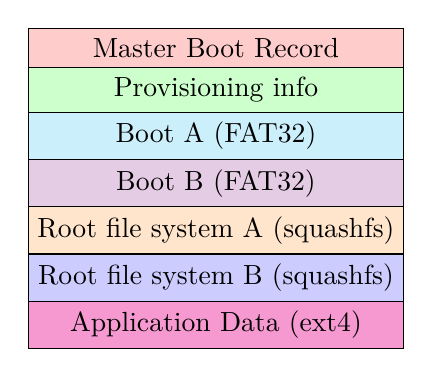
\begin{tikzpicture}
\node[rectangle split, rectangle split parts=7, rectangle split part fill={red!20,green!20,cyan!20,violet!20,orange!20,blue!20,magenta!40}, draw, black]
{Master Boot Record
\nodepart{two} Provisioning info
\nodepart{three} Boot A (FAT32)
\nodepart{four} Boot B (FAT32)
\nodepart{five} Root file system A (squashfs)
\nodepart{six} Root file system B (squashfs)
\nodepart{seven} Application Data (ext4)
};
\end{tikzpicture}
\end{center}
\end{frame}

\subsection{Logging}

\begin{frame}[standout]
\frametitle{\texttt{ring\_logger}}

{\color{white}
RingLogger is an in-memory ring buffer backend for the Elixir Logger with convenience methods for accessing the logs from the IEx prompt.

\faGithub \hspace{1pt} \href{https://github.com/nerves-project/ring_logger}{nerves-project/ring\_logger}
}
\end{frame}

\begin{frame}
  \frametitle{RingLogger use cases}

  \begin{itemize}
    \item Get log messages in real-time over remote IEx sessions
    \item Grep and tail through log messages without setting up anything else
    \item Keep logs in limited resource environments
    \item Capture recent log events for error reports
    \end{itemize}
  \end{frame}

\begin{frame}[fragile]
\frametitle{RingLogger usage sample}

\begin{example}
\begin{minted}[fontsize=\tiny,highlightlines={11,14}]{iex}
# env MIX\_TARGET=host iex --sname host1 --cookie hello -S mix
iex(host1@heimdallr)1> Logger.add_backend(:console)
{:ok, #PID<0.214.0>}
iex(host1@heimdallr)2> Logger.remove_backend(RingLogger)
:ok
iex(host1@heimdallr)3> require Logger
Logger
iex(host1@heimdallr)4> Logger.info("hello")
15:51:39.866 [info]  hello
:ok
iex(host1@heimdallr)5> Logger.add_backend(RingLogger)
{:ok, #PID<0.221.0>}
iex(host1@heimdallr)6> Logger.info("hello")
15:52:01.412 [info]  hello

:ok
\end{minted}
\end{example}

\begin{example}
\begin{minted}[fontsize=\tiny,highlightlines={2,5}]{iex}
# env MIX\_TARGET=host iex --sname host2 --cookie hello --remsh host1
iex(host1@heimdallr)1> RingLogger.attach()
:ok

15:52:01.412 [info]  hello
\end{minted}
\end{example}
\end{frame}

\begin{frame}[c,standout]
  \huge
  {
    \color{white} Phoenix Demo \\
    \large{\faGithub \hspace{1pt} \href{https://github.com/mobileoverlord/training_kiosk}{mobileoverlord/training\_kiosk}}
  }
\end{frame}

\begin{frame}[c,standout]
  \huge
  {\color{white} Questions?}
\end{frame}

\begin{frame}
\frametitle{More information}
\begin{itemize}
  \item
    \href{https://nerves-project.org/}{nerves-project.org}
  \item
    \href{https://embedded-elixir.com/}{embedded-elixir.com}
\item
    \href{https://hexdocs.pm/nerves}{hexdocs.pm/nerves}
\item
  \href{https://github.com/nerves-project}{github.com/nerves-project}
\item
  \href{https://github.com/nerves-hub}{github.com/nerves-hub}
\item
  \href{https://elixirforum.com/tags/nerves}{elixirforum.com/tags/nerves}
\item
  \href{https://elixir-slackin.herokuapp.com/}{elixir-slackin.herokuapp.com}
\item
  \href{https://github.com/nerves-project/nerves_examples}{github.com/nerves-project/nerves\_examples}
\end{itemize}
\end{frame}

\begin{frame}[c,standout]
  \huge
  {\color{white}Thanks! \\
    \large{Slides: \hspace{1pt} \href{https://speakerdeck.com/milmazz}{speakerdeck.com/milmazz}}
  }
\end{frame}
\end{document}
